%!TEX root =../project.tex
\part{Testing}
\section{Starting the program}
\paragraph{Expected Outcome} 
Two windows will open, the graphical output of the simulation and a menu. The
simulation should start running automatically. 
\paragraph{Actual Outcome} 
The program started as expected.
\begin{figure}[H]
	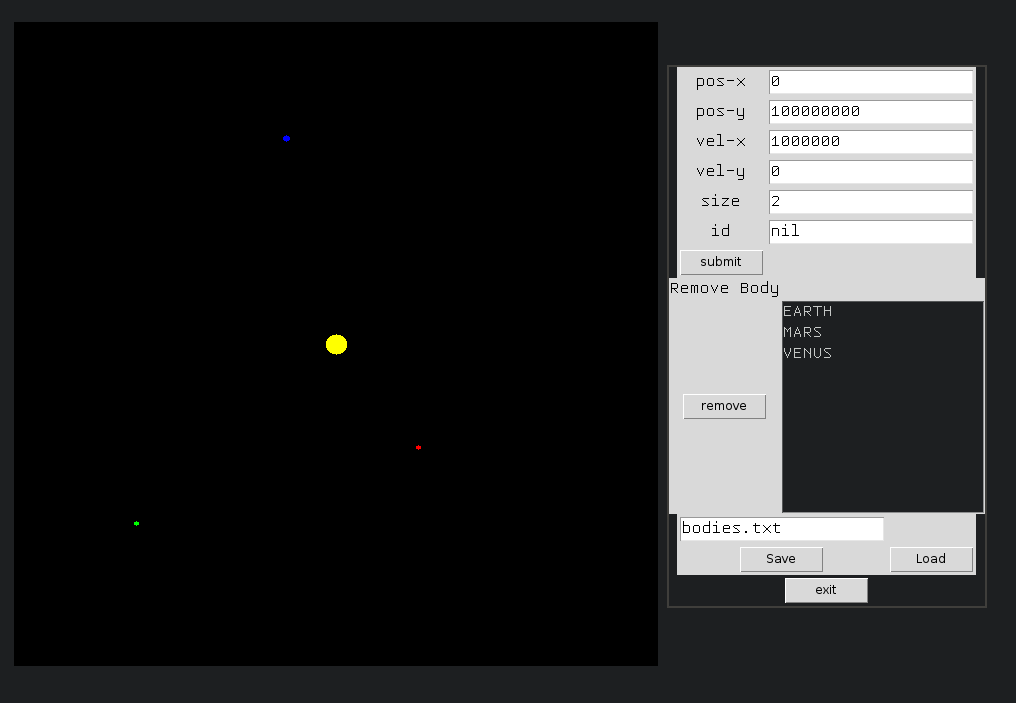
\includegraphics[width=\textwidth]{./img/start.png}
\end{figure}

\section{Closing the program}
\paragraph{Expected Outcome}
When the exit button is pressed, both the simulation window and the menu window
will close and no other messages will appear.
\paragraph{Actual Outcome}

\section{Running the simulation}
\subsection{Typical}
\paragraph{Expected Outcome}
The planets will orbit the sun on their respective paths, the patterns should be
repetitive and should not change.
\paragraph{Actual Outcome}
The planets all move along their expected paths, with no problems.

\subsection{Extreme}
\paragraph{Expected Outcome}
The planets will orbit the sun on their respective paths, the patterns should be
repetitive and should not change.
\paragraph{Actual Outcome}
The simulation continues to run despite having a lot more bodies than should be
needed, some of which were off the screen.
\begin{figure}[H]
	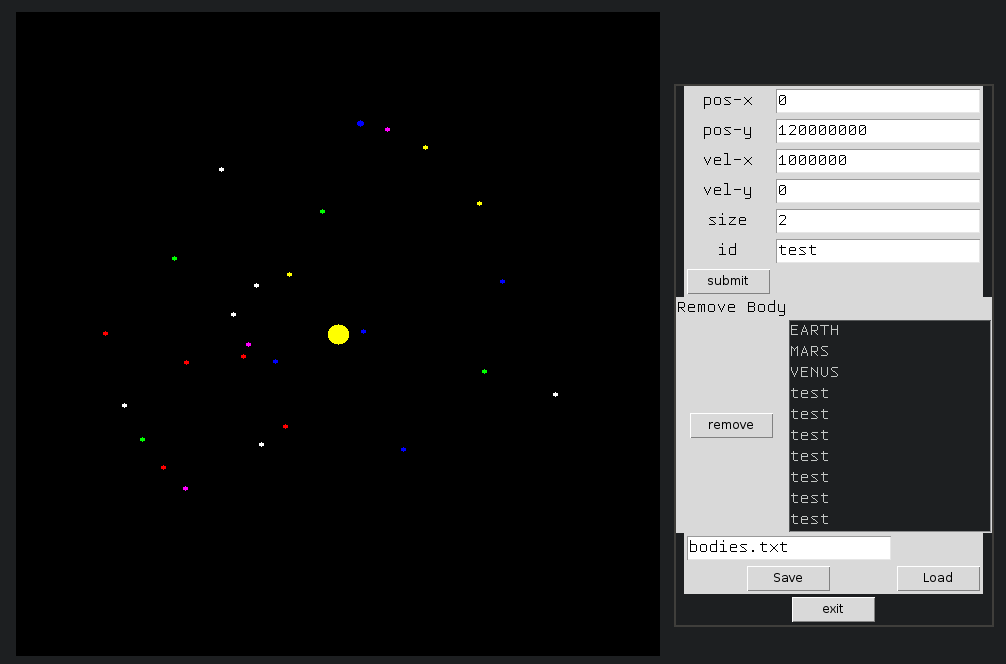
\includegraphics[width=\textwidth]{./img/run.png}
\end{figure}


\section{Adding a body}
\subsection{Typical}
\paragraph{Expected Outcome}
The body will be added to the simulation and it will follow its path, which
depends on the parameters it was added with.
\paragraph{Actual Outcome}
The body is added with the given parameters, and follows the path of its orbit.
\begin{figure}[H]
	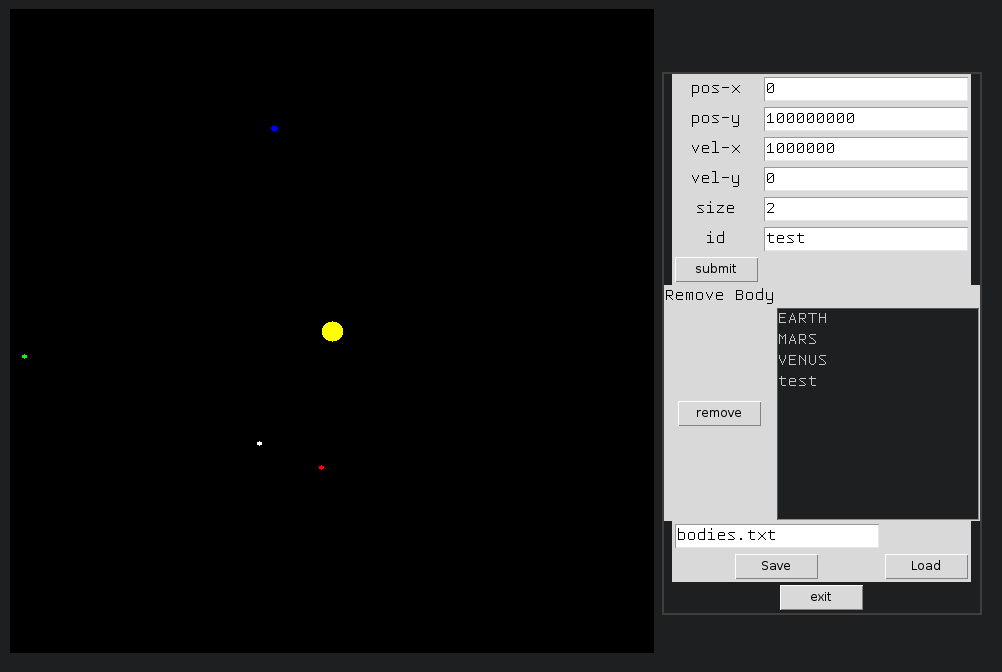
\includegraphics[width=\textwidth]{./img/add1.png}
\end{figure}

\subsection{Erroneous}
\paragraph{Expected Outcome}
A message box will appear to tell the user that the parameters given are not
valid, and should be changed.
\paragraph{Actual Outcome}
A message box appears warning the user, however the system still adds the body
with the erroneous value, causing the program to crash.
\begin{figure}[H]
	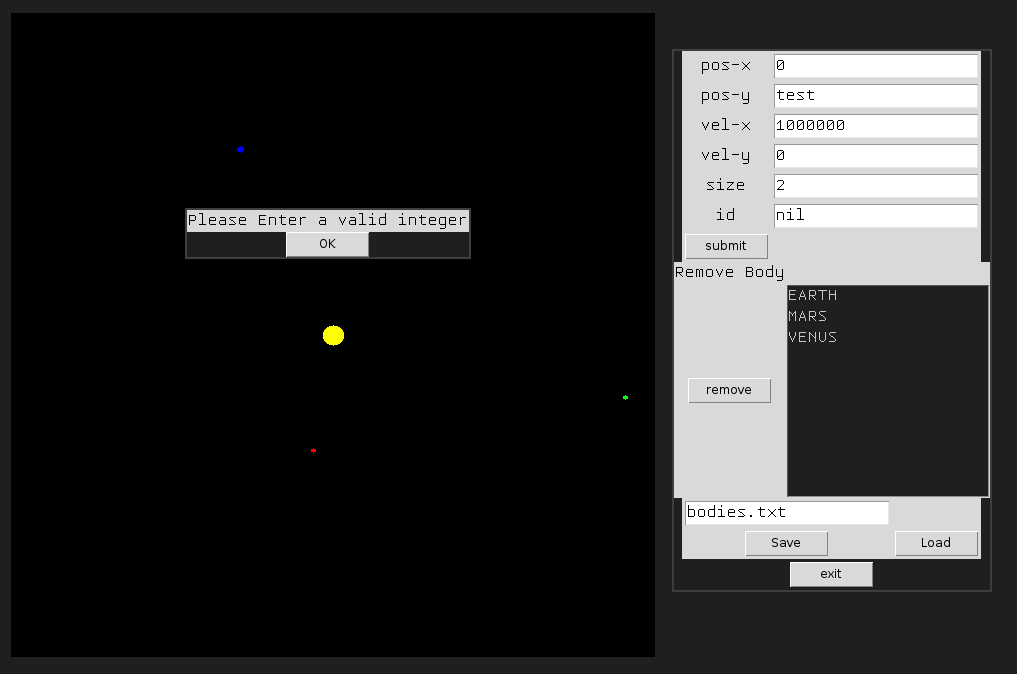
\includegraphics[width=\textwidth]{./img/add2.png}
\end{figure}
\paragraph{Comments and Corrective actions}
The code before initially was this lambda function that is called when the
submit button is pressed. 
\begin{lstlisting}
	(lambda ()
	   (apply #`add-body
		  (append
		   (mapcar #`parse-int
			   (list
			    (ltk:text in-posx)
			    (ltk:text in-posy)
			    (ltk:text in-velx)
			    (ltk:text in-vely)))
		   (list :size (parse-int (ltk:text in-size))
			 :id (ltk:text in-id)
			 :colour `a)))
	   (listbox-update bod-list))
\end{lstlisting}
And parse-int looked like this:
\begin{lstlisting}
(defun parse-int (str)
  "Converts a string to an int, and creates an error message if its invalid"
  (let ((int (parse-integer str :junk-allowed `t)))
    (if int
	int
	(error-message "Please Enter a valid integer"))))
\end{lstlisting}
As you can see, it does check if parse-integer return a valid answer, but the
only error handling it did was to create a message for the user. I created a
condition and had parse-int call it when it calls an error message.
\begin{lstlisting}
(define-condition invalid-input (error)
  ((str :initarg :str :reader str)))

(defun parse-int (str)
  "Converts a string to an int, and creates an error message if its invalid"
  (let ((int (parse-integer str :junk-allowed `t)))
    (if int
	int
	(progn (error-message "Please Enter a valid integer")
	       (error `invalid-input :str int)))))
\end{lstlisting}
However the lambda function that's called when the button is pressed still needs
to handle the error. The way to do this would be to have a return-from called
when the error is signalled but this requires the block that it is returning
from to be named, and this one isn't, so we have to wrap the contents of the
lambda function in a named block. The lambda is now:
\begin{lstlisting}
	(lambda ()
	   (block submit
	     (apply #`add-body
		    (append
		     (mapcar #`(lambda (x)
				 (handler-case
				     (parse-int x)
				   (invalid-input ()
				     (return-from submit `nil))))
			     (list
			      (ltk:text in-posx)
			      (ltk:text in-posy)
			      (ltk:text in-velx)
			      (ltk:text in-vely)))
		     (list :size (handler-case 
		     	             (parse-int (ltk:text in-size))
				   (invalid-input ()
				     (return-from submit `nil)))
			   :id (ltk:text in-id)
			   :colour `a)))
	     (listbox-update bod-list)))
\end{lstlisting}
I've added handler cases to everywhere that I've called parse-int, and they
break from the block when they detect the invalid-input error.
\subsection{Extreme}
\paragraph{Expected Outcome}
A message box will appear to tell the user that the values given could cause
problems with the simulation, and it is advised that they change them.
\paragraph{Actual Outcome}
The Body is added regardless.
\paragraph{Comments and Corrective actions}
I've added extra optional arguments to parse-int that allow you to pass in a min
and/or a max value for the number, and it will signal an error and create an
error message if the value is outside of these.
\begin{lstlisting}
(defun parse-int (str &key min max)
  "Converts a string to an int, and creates an error message if its invalid"
  (let ((int (parse-integer str :junk-allowed `t)))
    (if int
	(if (or (and (and min max) (> int min) (< int max))
		(and min (> int min))
		(and max (< int max)))
	    int
	    (progn (error-message "Please enter a valid integer")
		   (error `invalid-input)))
	(progn (error-message "Please enter a valid integer")
	       (error `invalid-input)))))
\end{lstlisting}
And the minimum and maximum values for different parameters are passed into
parse-int when it is called later.

\section{Removing a body}
\subsection{Typical}
\paragraph{Expected Outcome}
The selected body will be removed from the simulation.
\paragraph{Actual Outcome}
The selected body is removed from the simulation.
\begin{figure}[H]
	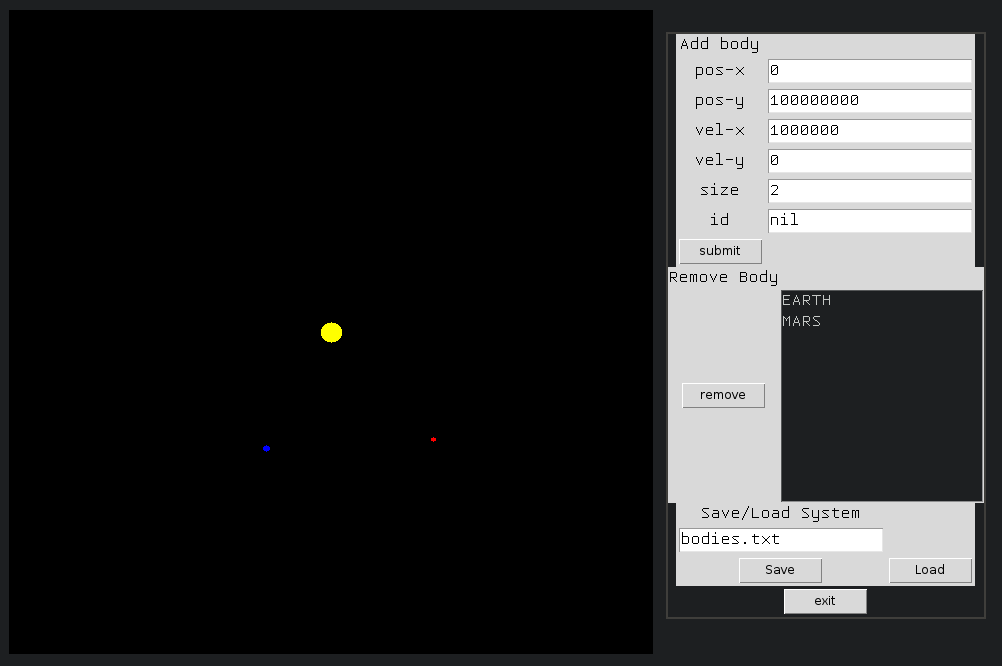
\includegraphics[width=\textwidth]{./img/rm.png}
\end{figure}

\subsection{Erroneous}
\paragraph{Expected Outcome}
A message box will appear to tell the user that they need to select a body
before they can remove one.
\paragraph{Actual Outcome}
A technical error message from LTK appearers, aimed at the programmer.
\begin{figure}[H]
	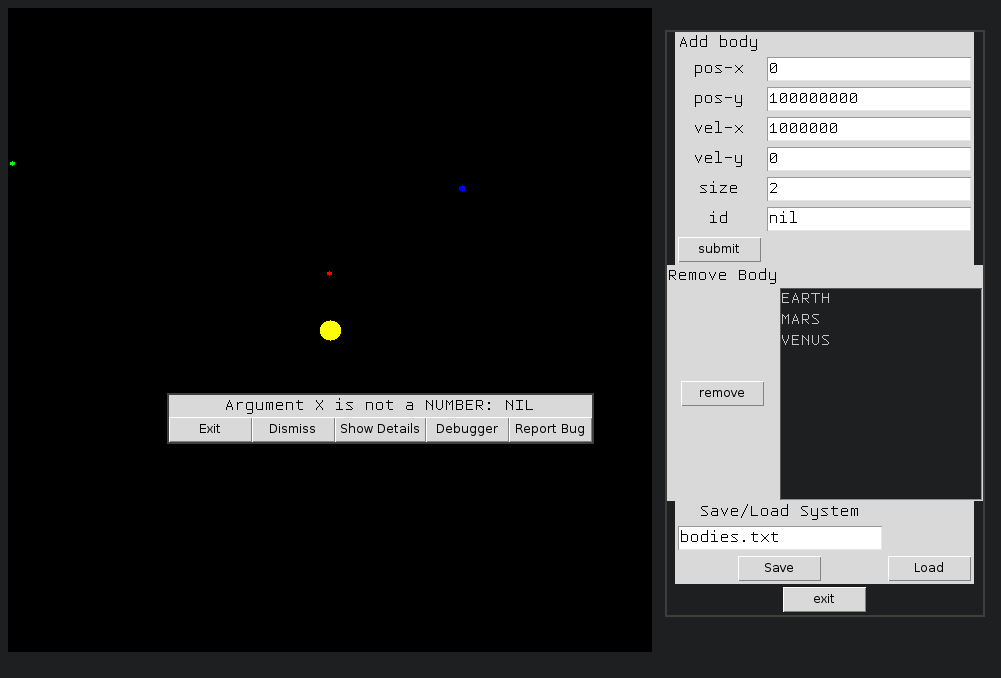
\includegraphics[width=\textwidth]{./img/rm2.png}
\end{figure}
\paragraph{Comments and Corrective actions}


\section{Saving the system to a file}
\subsection{Typical}
\paragraph{Expected Outcome}
The current details of the simulation will be saved to a file, with the name
given by the user.
\paragraph{Actual Outcome}
\paragraph{Comments and Corrective actions}

\subsection{Erroneous}
\paragraph{Expected Outcome}
A message box will appear to tell the user that the file name they have entered
is not valid, and should be changed before saving.
\paragraph{Actual Outcome}
\paragraph{Comments and Corrective actions}

\subsection{Extreme}
\paragraph{Expected Outcome}
The current details of the simulation will be saved to a file, with the name
given by the user.
\paragraph{Actual Outcome}
\paragraph{Comments and Corrective actions}


\section{Loading the system from a file}
\subsection{Typical}
\paragraph{Expected Outcome}
The details of the saved simulation will be loaded from the given file and will
replace the current system.
\paragraph{Actual Outcome}
\paragraph{Comments and Corrective actions}

\subsection{Erroneous}
\paragraph{Expected Outcome}
A message box will appear to tell the user that the file name they have entered
is invalid, or does not exist, and that they should enter a new one.
\paragraph{Actual Outcome}
\paragraph{Comments and Corrective actions}

\subsection{Extreme}
\paragraph{Expected Outcome}
The details of the saved simulation will be loaded from the given file and will
replace the current system.
\paragraph{Actual Outcome}
\paragraph{Comments and Corrective actions}


